%%%%%%%%%%%%%%%%%%%%%%%%%%%%%%%%%%%%%%%%%%%%%%%%%%%%%%%%%%%%%%%%%%%%%%%%%%%%%%%%%
\section{Inleiding}
\emph{Redirected walking} is een techniek waarbij een proefpersoon in een 
virtuele omgeving weergegeven in een head-mounted display kan rondwandelen door 
middel van het vervormen van de route die deze proefpersoon in een fysieke 
omgeving wandelt. Het doel is, door de 1:1 relatie van fysieke beweging en 
virtuele beweging te ontkoppelen, rondwandelen in grotere tot zelfs arbitrair 
grote virtuele ruimtes mogelijk te maken. Ik zal diverse technieken bespreken die
gebruikt worden om deze ontkoppeling teweeg te brengen. Naast de
redirectietechnieken zijn er ook technieken die de immersie verbeteren door
andere zintuigen te betrekken bij het proces. Dit heel proces wordt mogelijk 
gemaakt door een tracking systeem om een koppeling tussen de fysieke locatie van 
de proefpersoon en de locatie van zijn avatar in de virtuele omgeving mogelijk te
maken. Deze tracking systemen zullen ook kort worden besproken.


%%%%%%%%%%%%%%%%%%%%%%%%%%%%%%%%%%%%%%%%%%%%%%%%%%%%%%%%%%%%%%%%%%%%%%%%%%%%%%%%%
\section{Redirectietechnieken}
Om fysieke bewegingen door een virtuele omgeving mogelijk te maken wordt er
gebruik gemaakt van tracking systemen. Dit zijn systemen die bijvoorbeeld
camera's gebruiken om een koppeling te cre\"eren tussen de fysieke locatie van
een proefpersoon en de positie van zijn avatar in de virtuele omgeving. Omdat
deze trackingsystemen een tracking gebied hebben, het gebied waarbinnen ze de
locatie van de persoon kunnen waarnemen, is het nodig om technieken toe te passen
die de proefpersoon er van weerhouden dit gebied te verlaten.

Redirectietechniieken zijn technieken waar de fysieke bewegingen van een 
proefpersoon ontkoppeld worden van de resulterende virtuele bewegingen. Dit kan 
bijvoorbeeld gebeuren door de snelheid van de proefpersoon in de virtuele 
omgeving te versnellen of te vertragen ten opzichte van de snelheid in de fysieke
omgeving, of door de rotaties te vertragen of te versnellen zodat de proefpersoon
het tracking gebied niet verlaat. Ik bespreek hier enkele technieken: Het 
vervormen van buigingen en rotaties (Paragraaf \ref{1:rotation}), het vervormen van 
de lineaire snelheid van de proefpersoon (Paragraaf \ref{1:trans}), afleiders om
een route door de virtuele omgeving te forceren (Paragraaf \ref{1:distraction}) 
en verandering in de virtuele omgeving om een route in de fysieke omgeving te
forceren (Paragraaf \ref{1:blindness}).


\subsection{Rotationele vervorming} \label{1:rotation}
Bij rotationele vervorming worden de rotaties van de proefpersoon in de 
virtuele omgeving vergroot of verkleind ten opzichte van de rotaties van de 
proefpersoon in de fysieke omgeving, een voorbeeld hiervan kan men zien in Figuur 
\ref{fig:kohn01-movement}. In het algemeen is het hier het doel om de
proefpersoon indien mogelijk steeds richting het midden van de tracking area
te doen wandelen.

\begin{figure}[t!]
    \centering
    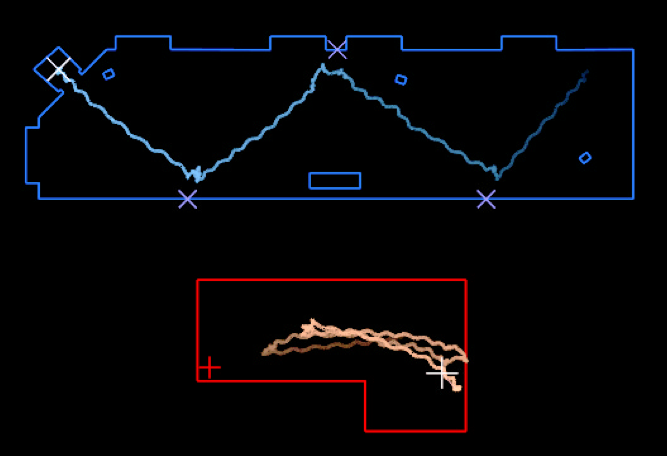
\includegraphics[width=0.7\textwidth]{kohn01-movement}
    \caption{Vergelijking van de beweging van de proefpersoon in de virtuele
    omgeving (bovenenaan) en de overeenkomstige beweging in de fysieke omgeving 
    (onderaan).\cite{kohn01}}
    \label{fig:kohn01-movement}
\end{figure}

Deze techniek is al in diverse papers onderzocht:

In een onderzoek gevoerd door Razzaque et. al., 2001 \cite{kohn01} werden 
proefpersonen gevraagd om een virtuele brandoefening uit te voeren. In de 
opstelling voor dit onderzoek waren er in het fysieke labo twee knoppen geplaatst
op dezelfde afstand als in de virtuele omgeving. In de virtuele omgeving waren er
echter 4 knoppen met telkens een hoek van 90 graden er tussen, deze opstelling is
in bovenaanzicht getoond in Figuur \ref{fig:kohn01-movement}. In dit onderzoek
werd op enkele verschillende manieren rotationele vervorming ingevoegd:

Als de proefpersoon stilstaat werd er een kleine hoeveelheid drift toegevoegd, 
dit deed men door de camera in de virtuele omgeving automatisch zeer traag in de 
omgekeerde richting van waar men de proefpersoon in de fysieke omgeving heen 
wilde naar laten kijken te laten draaien. Het bleek dat de proefpersoon hierdoor 
automatisch in die richting ging draaien om het beeld stil te houden. Omdat dit 
een zeer kleine (de precisie hoeveelheid werd niet gegeven) vervorming was, 
merkte de proefpersoon deze niet. De rotaties van de proefpersoon werden ook 
overdreven, of juist gedempt, om de proefpersoon in de fysieke omgeving in de 
juiste richting te laten wandelen.

Naast deze vervormingen indien de testpersoon in stilstand was, was het ook
mogelijk om een schijnbaar rechte lijn in de virtuele omgeving overeen te laten
komen met een curve. Dit effect werd bekomen door het pad in de virtuele omgeving
een bepaalde hoeveelheid te buigen, proportioneel met de lineaire snelheid van
de proefpersoon in de fysieke omgeving. Deze vervorming kan, in tegenstelling tot
de drift, enkel toegepast worden als de proefpersoon in beweging is.

Een combinatie van deze methodes werd gebruikt om er voor te zorgen dat als de
proefpersoon in de fysieke omgeving voor een knop stond, dit in de virtuele
omgeving ook het geval was. Helaas was het voor deze implementatie nodig dat er
een voorberekend pad door de virtuele omgeving bestond, en dat de proefpersoon
er zo weinig mogelijk van afweek.

Om deze vereiste van een statisch pad te ontwijken werd er in In Engel et. al., 
2008 \cite{engel08} een techniek voorgesteld om deze rotationele vervorming 
dynamisch te bepalen, dus de rotatie werd niet meer vervormd om een statisch pad
te volgen, maar om ten alle tijde in het tracking gebied te blijven. Dit werd 
gedaan door het dynamische-rotatie probleem te reduceren tot een optimisatie 
probleem, welke in de AI gemeenschap reeds bekend zijn. Dit algoritme maakte het 
mogelijk om optimale rotationele vervormingen te berekenen. Dit onderzoek 
verzwakte de limitering van een volledig statisch pad, naar een dynamisch pad in 
een gekende omgeving met voldoende bochten.

Om de limitering nog verder te verzwakken, werd er in een ander onderzoek in Neth 
et. al., 2012 \cite{neth12} verder onderzocht wat de precieze relatie tussen 
bewegingssnelheid en maximaal acceptabele rotationele vervorming is. Uit dit 
onderzoek bleek dat tragere snelheden grotere vervormingen toelaten, maar dat 
deze relatie niet lineair is, de relatie is exponentieel. Dit kan toegepast 
worden om de hoeveelheid geforceerde correcties (zie Paragraaf \ref{1:rot}) die
vereist zijn bij een willekeurige virtuele omgeving te verminderen.

In een tweede experiment uit hetzelfde onderzoek \cite{neth12} werd onderzocht 
of deze bevindingen effectief konden gebruikt worden om dynamische schalering van 
vervorming toe te passen in een rijke virtuele omgeving. Er werd hier onderzocht 
of er een significant verschil is tussen de merkbaarheid van statische 
rotationele vervorming (als de proefpersoon stil staat) versus dynamische 
rotationele vervorming (als de proefpersoon beweegt). Naast de technieken van 
Razzaque et. al., 2001 \cite{kohn01} om rotationele vervorming in te voegen met 
een constant, een statisch en een dynamisch component, werd er ook gebruik 
gemaakt van versterking van de effecten nabij de randen van de fysieke omgeving, 
om het verlaten van het tracking gebied te vermijden. 

Er werd gemeten wat de mediaanafstand is die een proefpersoon kan wandelen in een 
grote virtuele omgeving voor de proefpersoon moet geforceerd geherori\"enteeerd 
worden richting het centrum van de fysieke omgeving om het verlaten van het 
tracking gebied te voorkomen. Uit dit experiment is gebleken dat er een positief 
significant verschil is tussen de mediaan gewandelde afstand bij dynamische 
vervorming (de hoeveelheid vervorming is afhankelijk van de wandelsnelheid) 
versus de mediaan gewandelde afstand bij statische vervorming (de hoeveelheid
vervorming wordt niet aangepast aan de wandelsnelheid).

In deze studies werd enkel gekeken naar rotationele vervorming in beweging, dus 
over curves. Het is echter ook mogelijk om rotationele vervorming in stilstand te
hebben. In Steinicke et. al., 2009 \cite{steinicke09} werd bepaald dat in dit 
specifieke geval compressies tot 77\% acceptabel zijn voordat de proefpersoon het 
merkt.

Uit al deze onderzoeken blijkt dat er een trade-off is tussen een virtuele 
omgeving met een ongekend pad\cite{neth12} versus een betere immersie wegens 
minder onderbrekingen\cite{engel08,kohn01}.


\subsection{Translationele vervorming} \label{1:trans}
Naast rotationele vervorming is het ook mogelijk om de lineaire snelheid van een
proefpersoon te vervormen daar onderzoek heeft aangetoond dat proefpersonen in 
virtuele omgevingen afstand \cite{loomis03}, snelheid \cite{banton05} en 
afgelegde afstand \cite{frenz07} onderschatten. In Steinicke et. al., 2009 \cite{steinicke09} 
werd er een experiment uitgevoerd om onder andere te bepalen wat de maximaal 
acceptabele translationele vervorming is voor een gegeven snelheid. Er werd 
bepaald dat de vervorming merkbaar is bij een versnelling tussen 20\% en 60\% 
met een ideale waarde van ongeveer 20\%.

Rotationele vervorming en translationele vervorming vormen de basis van
redirected walking zonder in te grijpen in de 3d scene. Ze zijn ook de twee 
technieken die gebruik maken van ontkoppeling van het fysieke en het virtuele 
pad van de proefpersoon.


\subsection{Change blindness} \label{1:blindness}
In de vorige technieken werd er enkel ingegrepen in de route door de virtuele
omgeving door de route door de fysieke omgeving te ontkoppelen van de route door
de virtuele omgeving. Het is echter ook mogelijk om in de route door de fysieke
omgeving in te grijpen door de 3d scene van de virtuele omgeving aan te passen.

Change blindness slaat op de manier waarop mensen onder bepaalde omstandigheden
verrassend grote veranderingen in een omgeving niet merken. In een paper van
Simons et. al., 2005 \cite{simons05} wordt er een breed overzicht gegeven van de
diverse experimenten die zijn uitgevoerd rond dit fenomeen. Zo merken veel mensen
bijvoorbeeld helemaal niet als een persoon in het midden van een interactie door
een totaal andere persoon wordt vervangen\cite{simons98}, of wordt het verschil
tussen twee foto's die om de beurt worden getoond (zie Figuur \ref{fig:pictures})
pas na een zeer lange tijd opgemerkt\cite{rensink97}.

\begin{figure}[t!]
    \centering
    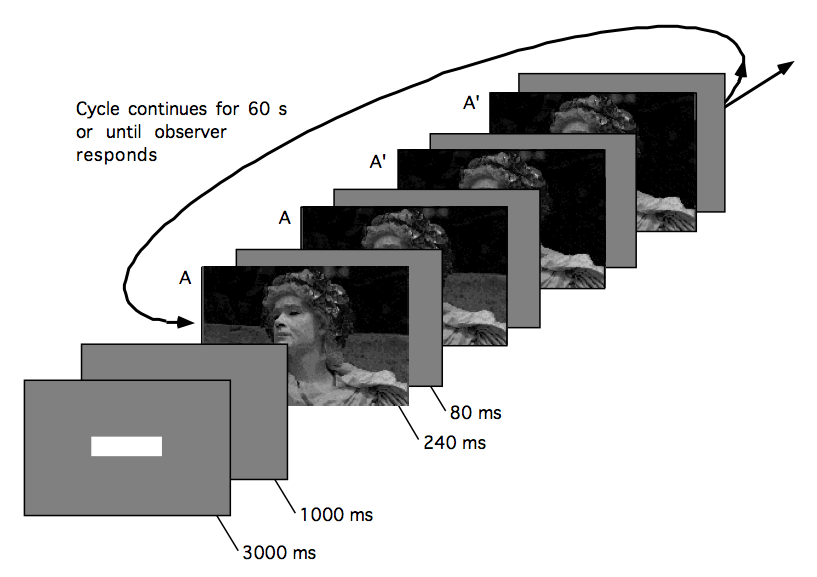
\includegraphics[width=0.7\textwidth]{pictures}
    \caption{Werkwijze voor het weergeven van 2 verschillende afbeeldingen, om te 
    kijken hoe snel mensen dit merken.\cite{rensink97}}
    \label{fig:pictures}
\end{figure}

Omdat dit zo een krachtig fenomeen is, wordt het ook toegepast in redirected 
walking. Waar de vorige technieken het fysieke en het virtuele pad van de 
proefpersoon ontknoppelden probeert deze techniek de proefpersoon te misleiden. 
Om er voor te zorgen dat hij in de tracking ruimte blijft, wordt de layout van de 
virtuele omgeving strategisch aangepast, bijvoorbeeld door een deur van
plaats te laten wisselen zoals in Figuur \ref{fig:suma1}.

\begin{figure}[t!]
    \centering
    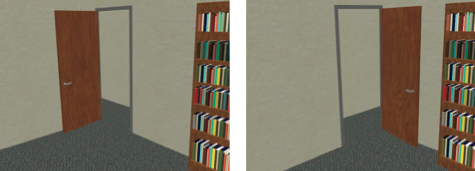
\includegraphics[width=0.7\textwidth]{suma1}
    \caption{Voorbeeld van een verandering in een virtuele omgeving, de deur
    werd hier van plaats veranderd terwijl de proefpersoon er niet naar aan het
    kijken was.\cite{suma11}}
    \label{fig:suma1}
\end{figure}

Zo werd er bijvoorbeeld in Suma et. al., 2011 \cite{suma11} getest of 
veranderingen in de virtuele omgeving voor de proefpersonen merkbaar waren. 
De proefpersoon werd gevraagd om in een virtueel kantoor in elke kamer een 
beeldscherm uit te zetten en vervolgens de kamer verlaten. Dit proces werd dan 
herhaald voor alle 16 kamers in het kantoor. De ingrijping in de omgeving
gebeurde hier terwijl de proefpersoon het scherm uitzette, en met zijn rug naar
de deur stond. De deur veranderde van positie zodat de gang in een hoek van 90 
graden verder ging ten opzichte van hoe de proefpersoon de kamer binnenkwam. 
Dit hele proces is zichtbaar in Figuur \ref{fig:suma2}.

\begin{figure}[t!]
    \centering
    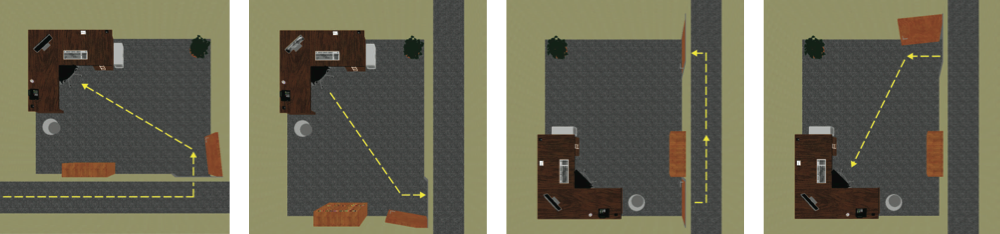
\includegraphics[width=\textwidth]{suma2}
    \caption{Verandering van de positie van de deur in het onderzoek van Suma et. 
    al., 2011 \cite{suma11}.}
    \label{fig:suma2}
\end{figure}

Door de veranderingen van de fysieke omgeving op deze manier te laten gebeuren
werd de proefpersoon geforceerd cirkels rond de tracking area te wandelen, in
Figuur \ref{fig:suma3} is een illustratie van het pad door de fysieke omgeving te
zien, overeenkomstig met het pad door een kamer in de virtuele omgeving.

\begin{figure}[t!]
    \centering
    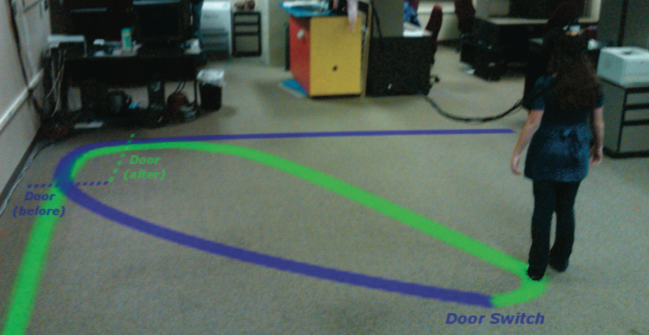
\includegraphics[width=0.7\textwidth]{suma3}
    \caption{Voorbeeld van het pad in de fysieke omgeving wegens de verandering
    in de virtuele omgeving, dit is het pad dat veroorzaakt werd door de 
    verandering in Figuur \ref{fig:suma2}.\cite{suma11}}
    \label{fig:suma3}
\end{figure}

Na de uitvoering van het experiment werd er een vragenlijst afgenomen, er is 
toen gemerkt dat deze verandering voor bijna iedereen compleet onmerkbaar was, en
werd er zelfs maar in kleine mate ervaren dat men in cirkels was aan het 
wandelen.


\subsection{Afleiders} \label{1:distraction}
Een laatste techniek die ik zal bespreken is het toevoegen van ``afleiders'',
dynamisch bewegende voorwerpen of personen die als doel hebben de proefpersoon
uit eigen wil zijn pad te laten afbuigen. Afleiders kunnen ook gebruikt worden
om de ontkoppelingen van het virtuele en het fysieke pad minder te laten 
opvallen.

In een onderzoek van Neth et. al., 2012 \cite{neth12} werd er bijvoorbeeld 
gebruik gemaakt van andere virtuele avatars zoals in Figuur \ref{fig:avatars}.
Er werd gebruik gemaakt van avatars die recht voor de proefpersoon gingen
stilstaan om hem te dwingen te vertragen indien hij te snel ging om het pad
effectief af te buigen. Er werd ook gebruik gemaakt van avatars die op koers
wandelden voor een botsing om de proefpersoon te forceren af te buigen.

\begin{figure}[h!]
    \centering
    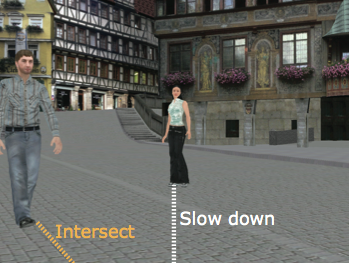
\includegraphics[width=0.7\textwidth]{avatars}
    \caption{Voorbeeld van het toevoegen van avatars in een virtuele omgeving, 
    met als doel de proefpersoon te laten vertragen of zijn pad af te 
    buigen.\cite{neth12}}
    \label{fig:avatars}
\end{figure}

In Peck et. al., 2009 \cite{peck09} werd er op een andere manier gebruik gemaakt 
van afleiders. Er werd gevraagd aan de proefpersoon om een vlinder te volgen om
hem de illusie te geven dat hij \mbox{360\textdegree} heeft gedraaid terwijl hij 
eigenlijk maar 180\textdegree{} heeft gedraaid. Hieruit bleek dat proefpersonen 
minder het gevoel hadden dat de wereld versneld draaide met een afleiding dan 
bij andere technieken.


%%%%%%%%%%%%%%%%%%%%%%%%%%%%%%%%%%%%%%%%%%%%%%%%%%%%%%%%%%%%%%%%%%%%%%%%%%%%%%%%%
\section{Reori\"entatietechnieken} \label{1:rot}
Hoewel redirectietechnieken bedoeld zijn om een proefpersoon binnen een tracking
area te laten wandelen, kan het soms gebeuren dat een botsing met de rand van de
tracking area niet meer te vermeiden is. Als dit het geval is moet de gebruiker
op een minder subtiele manier duidelijk gemaakt worden dat hij moet omkeren. Er 
wordt dan gebruik gemaakt van ``reori\"entatietechnieken''. Dit zijn directe 
commando's aan de proefpersoon om van koers te veranderen, en vallen daarom ook 
behoorlijk op. In de volgende secties bespreek ik twee reori\"entatietechnieken:
Het gebruik van verbale commando's (Paragraaf \ref{1:verbal}) en het gebruik van
visuele commando's (Paragraaf \ref{1:visual}).



\subsection{Verbale commandos} \label{1:verbal}
Bij verbale commandos wordt er een geluidssignaal gegeven (meestal een gesproken
signaal) waarin de proefpersoon wordt gevraagd om te draaien.

In het onderzoek van Razzaque et. al., 2001 \cite{kohn01} werd, indien de
proefpersoon dreigde het tracking gebied te verlaten, de proefpersoon met verbale
commando's gevraagd stil te staan en heen en weer te kijken om de proefpersoon in
de fysieke omgeving terug in de juiste richting te laten kijken.

Er werd in een andere studie van Peck et. al., 2009 \cite{peck09} echter bevonden 
dat verbale commando's niet de beste optie zijn voor redirectietechnieken, omdat
deze makkelijk genegeerd kunnen worden.


\subsection{Visuele commandos} \label{1:visual}
Bij visuele commandos wordt er een signaal op de display weergegeven om de 
proefpersoon te vragen om te draaien.

In het onderzoek van Neth et. al., 2012 \cite{neth12} werd onder andere gebruik 
gemaakt van een stopteken. Als dit werd getoond werd de hele virtuele wereld stil 
gelegd. Er werd op voorhand aan de proefpersoon gevraagd rond te draaien tot het 
stopteken verdwijnt indien het getoond werd. Hoewel dit een zeer intrusieve 
methode is, is ze zeer effectief om het verlaten van het tracking gebied te 
voorkomen daar ze niet te negeren is.


%%%%%%%%%%%%%%%%%%%%%%%%%%%%%%%%%%%%%%%%%%%%%%%%%%%%%%%%%%%%%%%%%%%%%%%%%%%%%%%%%
\section{Immersie}
Het is bij het wandelen door een virtuele omgeving belangrijk dat de gebruiker
zich voelt alsof hij echt in de virtuele omgeving is. Dit algemene gevoel wordt
immersie genoemd. Ik bespreek hier de invloed van de diverse zintuigen op
immersie.

Visie is voor redirected walking het belangrijkst. Dit komt omdat bij conflicten
tussen het proprioceptieve systeem (Het zintuig dat de relatieve afstand tussen
lichaamsdelen waarneemt), het vestibulaire systeem (Het zintuig verantwoordelijk 
voor ons evenwichtsgevoel) systeem en visie, visie vaak dit conflict 
wint\cite{berthoz02,dichgans78,bruder08}. Om immersie visueel te verkrijgen moet 
er gebruik gemaakt worden van head-mounted displays.

Ook al is visie het belangrijkste zijn de andere zintuigen toch belangrijk om 
immersie te verkrijgen. Als men in een virtuele omgevingen geluid realistisch kan 
positioneel reproduceren helpt dit bijvoorbeeld de immersie 
enorm\cite{lackner77}, maar zelfs het maskeren van geluid van in de fysieke 
wereld met bijvoorbeeld ruis kan helpen\cite{usoh99}. In Engel et. al., 
2008\cite{engel08} wordt ook opgemerkt dat de hoeveelheid omgevingslicht en 
omgevingsgeluid dat binnensijpelt een merkbare negatieve invloed heeft op de 
effectiviteit van redirectietechnieken. 

Het is ook mogelijk om de immersie te verhogen met haptische feedback. Dit wordt
gedaan met proxy-objecten in de fysieke omgeving die overeen komen met objecten 
in de virtuele omgeving\cite{steinicke09} zoals te zien is in Figuur 
\ref{fig:proxy-object}.

\begin{figure}[t!]
    \centering
    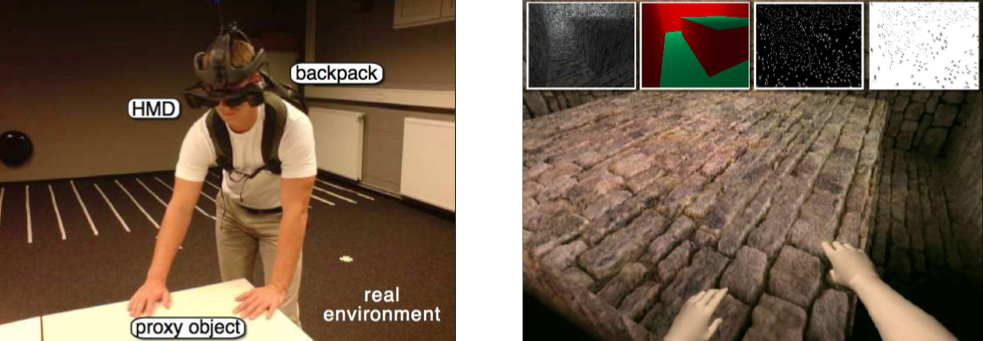
\includegraphics[width=0.7\textwidth]{proxy-object}
    \caption{Voorbeeld van een proxy-object en het overeenkomstige beeld dat de
    proefpersoon ziet.\cite{steinicke09}}
    \label{fig:proxy-object}
\end{figure}

Voor de effectieve weergave van de virtuele omgeving maakt men meestal gebruik 
van een head mounted display, of een HMD. Voor HMDs is het ideaal om een zo hoog 
mogelijke field of view te hebben, dit lijkt geen groot effect te hebben op het 
optreden van simulatieziekte\cite{arthur00} maar verhoogt de performantie en 
immersie drastisch\cite{arthur00}.

Hoewel redirected walking een realistische en immersieve omgeving kan cre\"eren 
zijn er toch enkele inherente zwaktes waar op zich niet omheen kan gewerkt 
worden. Zo is het bijvoorbeeld onmogelijk om arbitraire fysieke collisie overeen 
te laten komen met collisie in de virtuele omgeving tenzij het labo expliciet 
voor die virtuele omgeving is gebouwd. Het is ook niet mogelijk om de textuur van
de vloer in de fysieke omgeving overeen te laten komen met deze in de virtuele
omgeving als deze verandert van kamer tot kamer.

%%%% VERPLAATSEN NAAR OPSTELLING!!!
%Traditioneel waren HMDs met grote field of view zeer duur en niet beschikbaar voor
%consumenten, maar tegenwoordig zijn er enkele betaalbare HMDs beschikbaar met een
%redelijk grote field of view, zoals de Oculus Rift DK1 (110\textdegree{} 
%diagonaal).
%
%\begin{figure}[t!]
%    \centering
%    \includegraphics[width=0.7\textwidth]{or-dk1}
%    \caption{De Oculus Rift Developer Kit 1}
%    \label{fig:or-dk1}
%\end{figure}
%
%Ten laatste is het voor immersie ook belangrijk dat de positie van de 
%proefpersoon in de fysieke omgeving zeer precies geweten. Er zijn
%hier echter een grote hoeveelheid commerci\"ele systemen voor beschikbaar zoals
%het OptiTrack systeem.


%%%%%%%%%%%%%%%%%%%%%%%%%%%%%%%%%%%%%%%%%%%%%%%%%%%%%%%%%%%%%%%%%%%%%%%%%%%%%%%%%
\section{Conclusie}
Bij redirected walking is er een trade-off tussen dynamische en statische paden.
Bij dynamische paden is de immersie in de omgeving zeer hoog daar de gebruiker
niet geforceerd is een pad te volgen, maar aan de andere kant wordt de immersie
vaak gebroken omdat het systeem gedwongen is de gebruiker te laten omkeren. Aan 
de andere kant hebben statische paden weinig risico dat de gebruiker het
tracking gebied verlaat, maar wordt de gebruiker zijn immersie verminderd omdat
hij geforceerd een pad door de virtuele omgeving kan volgen.

Ergens in het midden van deze trade-off ligt change blindness. Het pad is 
statisch, want er wordt verwacht dat de gebruiker de kamers op een bepaalde
volgorde doorloopt. Maar in de kamers zelf maakt het gekozen pad niet uit, want
de virtuele omgeving is zo gemanipuleerd dat de gebruiker het tracking gebied
niet zomaar kan verlaten. Maar change blindness vereist op zich dat de virtuele
omgeving zeer specifiek met het tracking gebied in gedachte moet opgebouwd 
worden.

Juist omdat change blindness in het midden van deze trade-off ligt heb ik ervoor
gekozen om dit verder te onderzoeken. Beide extremen brengen veel problemen met
zich mee, en hoewel change blindness een zeer specifieke virtuele omgeving
vereist denk ik dat hier toch heel veel mee gedaan kan worden.

Voor deze bachelorproef zal ik een experiment uitvoeren om te kijken hoe 
merkbaar change blindness met afleiders en taken is in een virtuele omgeving.